\section{Methodology}
\begin{figure*}[t]
    \centering
    \scalebox{0.28}{
    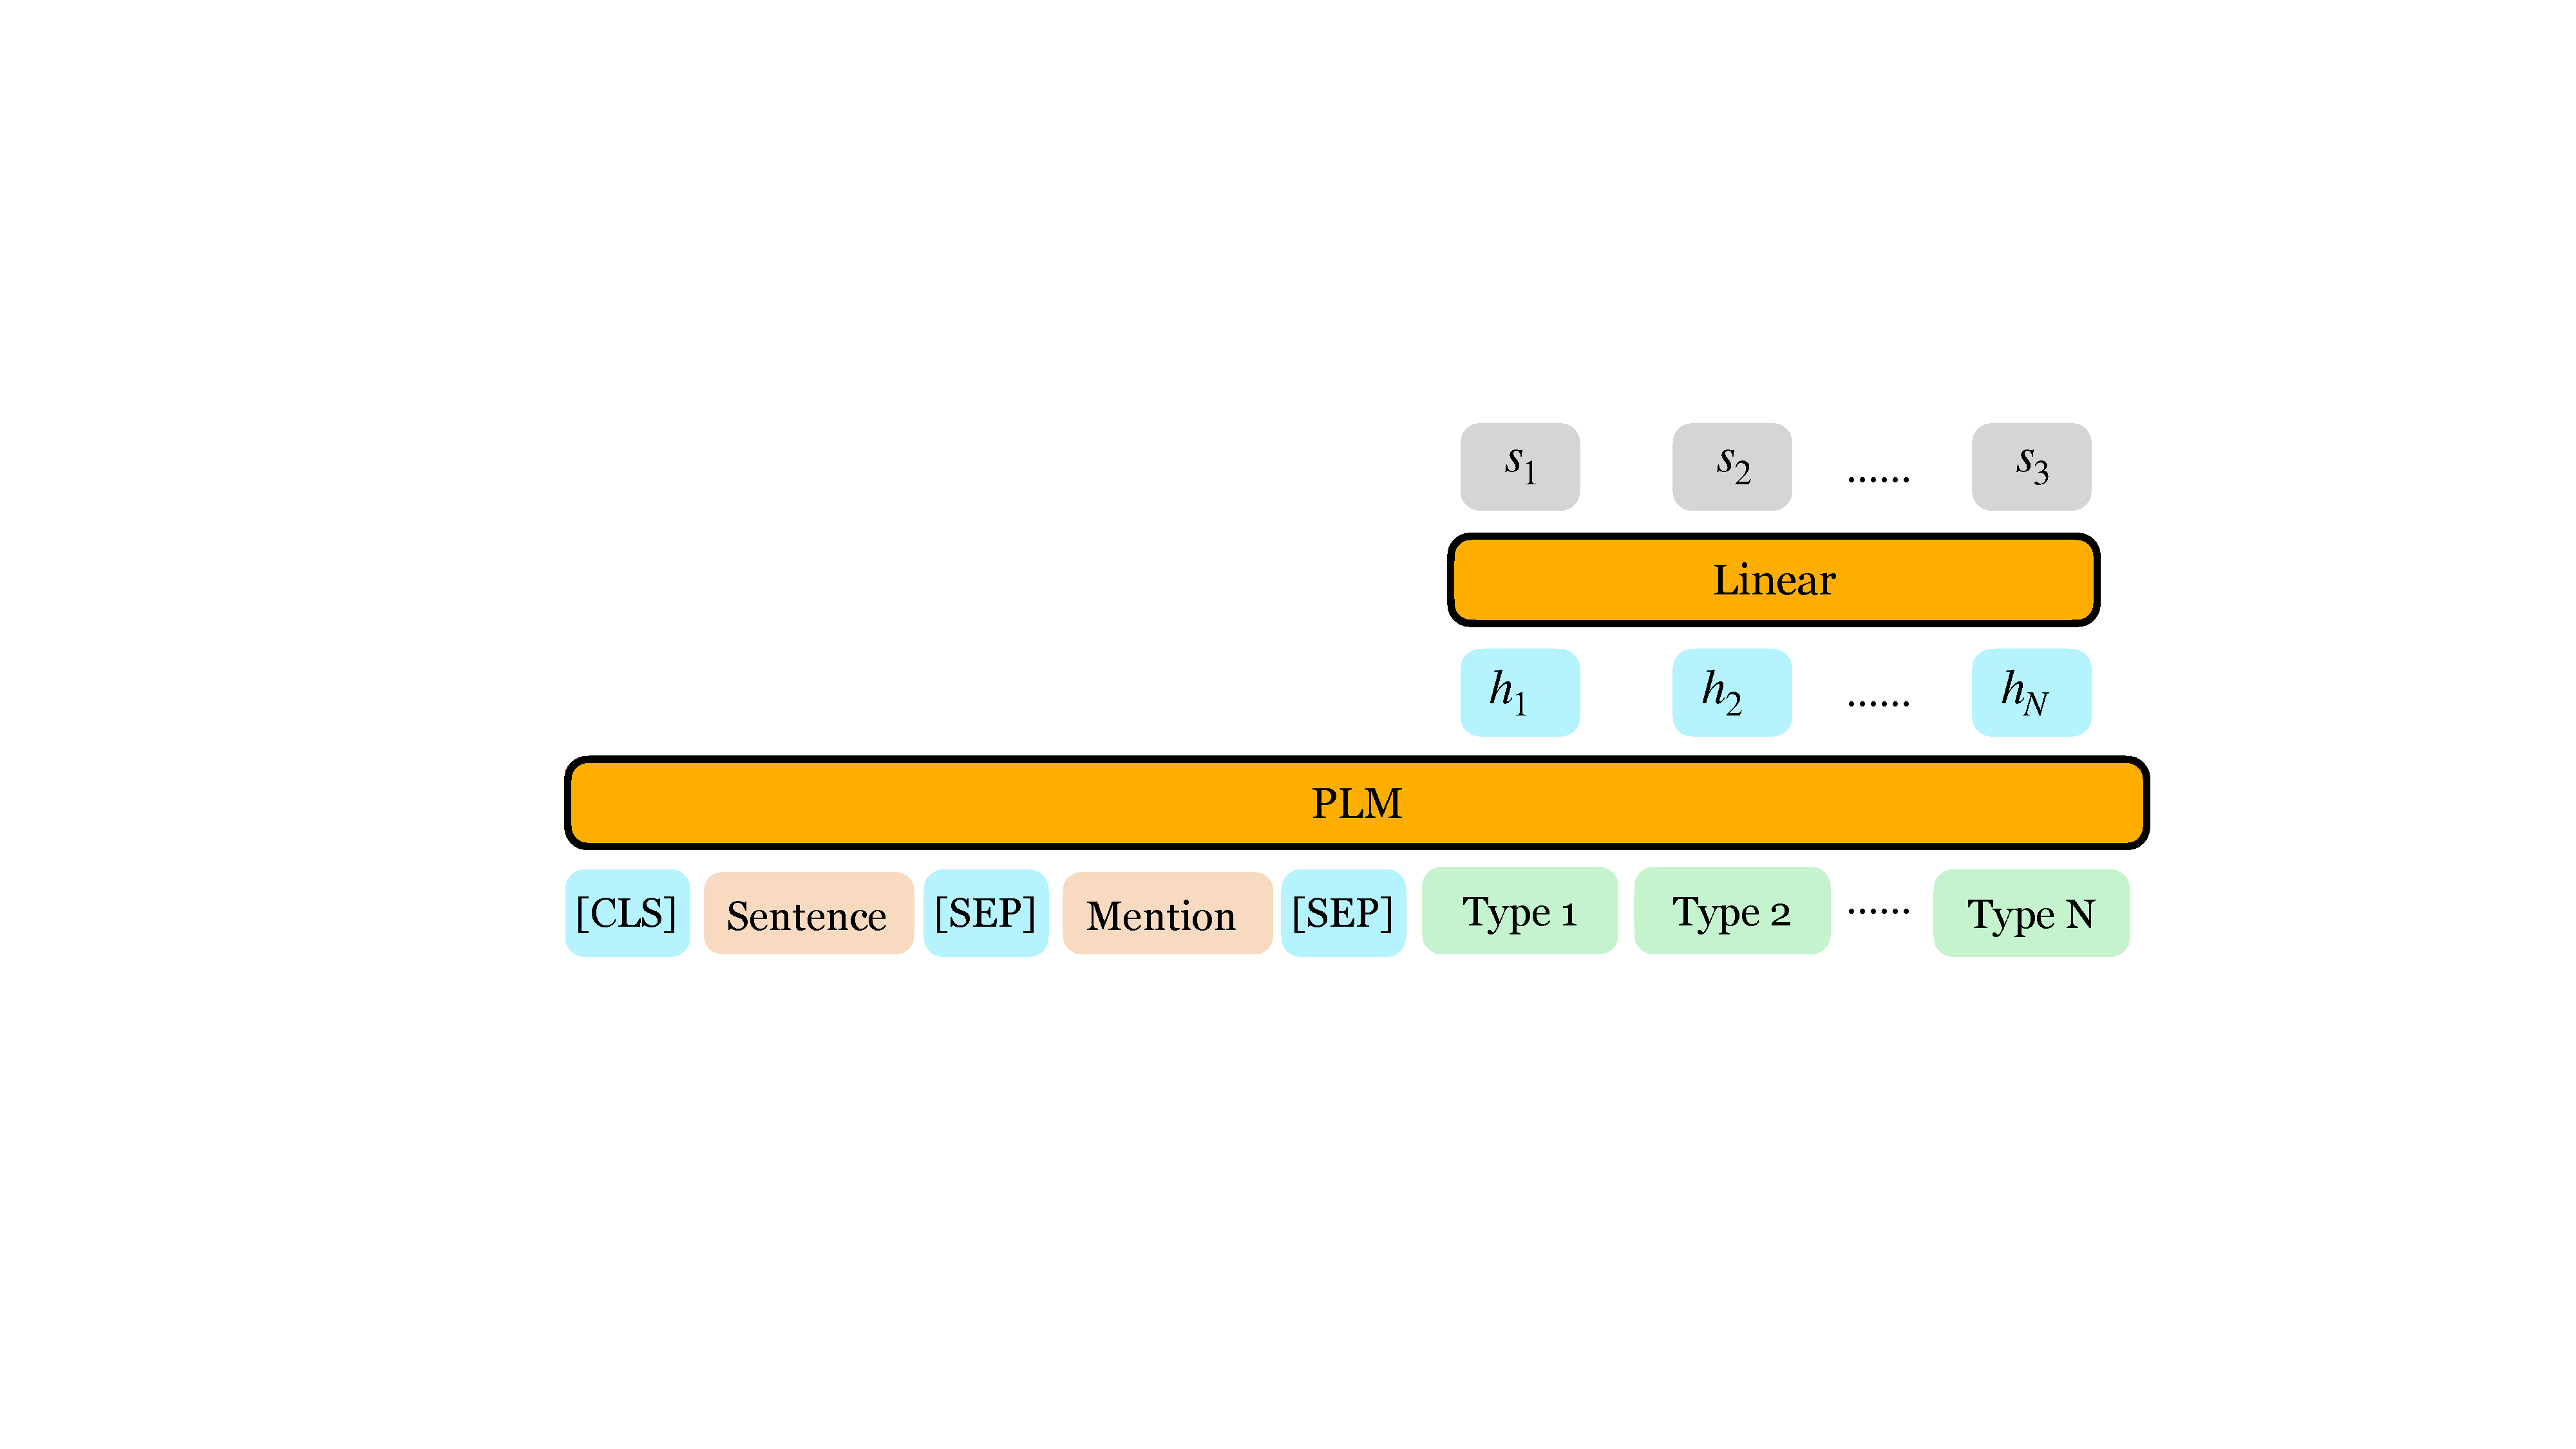
\includegraphics{src/img/ccf_model.pdf}}
    \caption{Multi-candidate cross-encoder (MCCE).}
    \label{fig:ccf}
\end{figure*}
Inspired by techniques in information retrieval \cite{ir} and entity linking \cite{wu2019zero}, we decompose the training and inference of UFET into three stages as illustrated in Figure \ref{fig:paradigm}: (1) Recall stage to reduce the type candidate size (e.g., from $N=10k$ to $K=100$) while guaranteeing the recall rate by an efficient MLC model. (2) Expand stage to incorporate lexical information using exact matching and weak supervision \cite{mlmet} from large pretrained language models such as BERT-Large \cite{bert} to improve recall rate. (3) Filter stage to filter the expanded type candidates to obtain final prediction. For the filter stage, we propose an efficient model: Multi-Candidate Cross-Encoder (MCCE) to concurrently encode and filter type candidates of a given mention with only a single forward pass. 
\subsection{Recall Stage}
To prune the type candidates set, we train a very efficient MLC model introduced in Sec. \ref{sec:mlc} and select the model based on the recall rate (e.g. recall@64) on the development set. Then we use it to infer the top $K_1$ (typically less than 256) candidates $\mathcal{C}_i^R$ for each data point $(m_i, c_i)$ for train, development, and test set. We compare MLC with a widely-used baseline model BM25 \cite{bm25} and show its advantages in Sec. \ref{sec:recall}. 
% There are other options (e.g., Bi-Encoder \cite{wu2019zero}) for the recall model. However, we choose MLC because it is easy to optimize and has the fastest inference speed\footnote{MLC model can be categorized as a simple Bi-Encoder that uses embedding to encode types.}.
\subsection{Expand Stage}
Due to the lack of training data per type, we found that the MLC we used in the recall stage easily overfits the train set, and is hard to predict the types that only appear in the development and test set. In {\bf \textsc{UFET}} dataset, 30\% of the types in the development set are unseen. To this end, we utilize lexical information using exact match and weak supervision from the masked language model (MLM) to expand the recalled candidates. Both exact match and MLM are able to recall unseen type candidates without any training. 
\paragraph{Exact Match} MLC and Bi-Encoder recall candidates by dense representations. They are known weak at identifying and utilizing the lexical matching information between the input and types \cite{matching_info1, matching_info2}. However, 
 types are free-formed in UFET (e.g., \textit{president, businessman}), and are very likely to appear in the context or mention (e.g., the mention is \textit{`the \textbf{president} Joe Biden'}). To this end, we first find all nouns in the context and mention by NLTK\footnote{nltk.tag package \url{https://www.nltk.org}} POS tagger and normalize their forms, then we recall types that exactly matched with these nouns.
\paragraph{Weak Supervision from MLM} Inspired by recently prompt-based methods for entity typing \cite{ding2021prompt, dfet}, we recall candidates by asking PLMs to fill masks in prompts. Suppose a type $y_j \in \mathcal{Y}$ can be tokenized into $l$ subwords $w_1, \cdots w_l$. To score $y_j$ given $m_i, c_i$, we first formulate the input as in Figure \ref{fig:prompt_recall}.
\begin{figure}[h]
    \centering
    \scalebox{0.2}{
    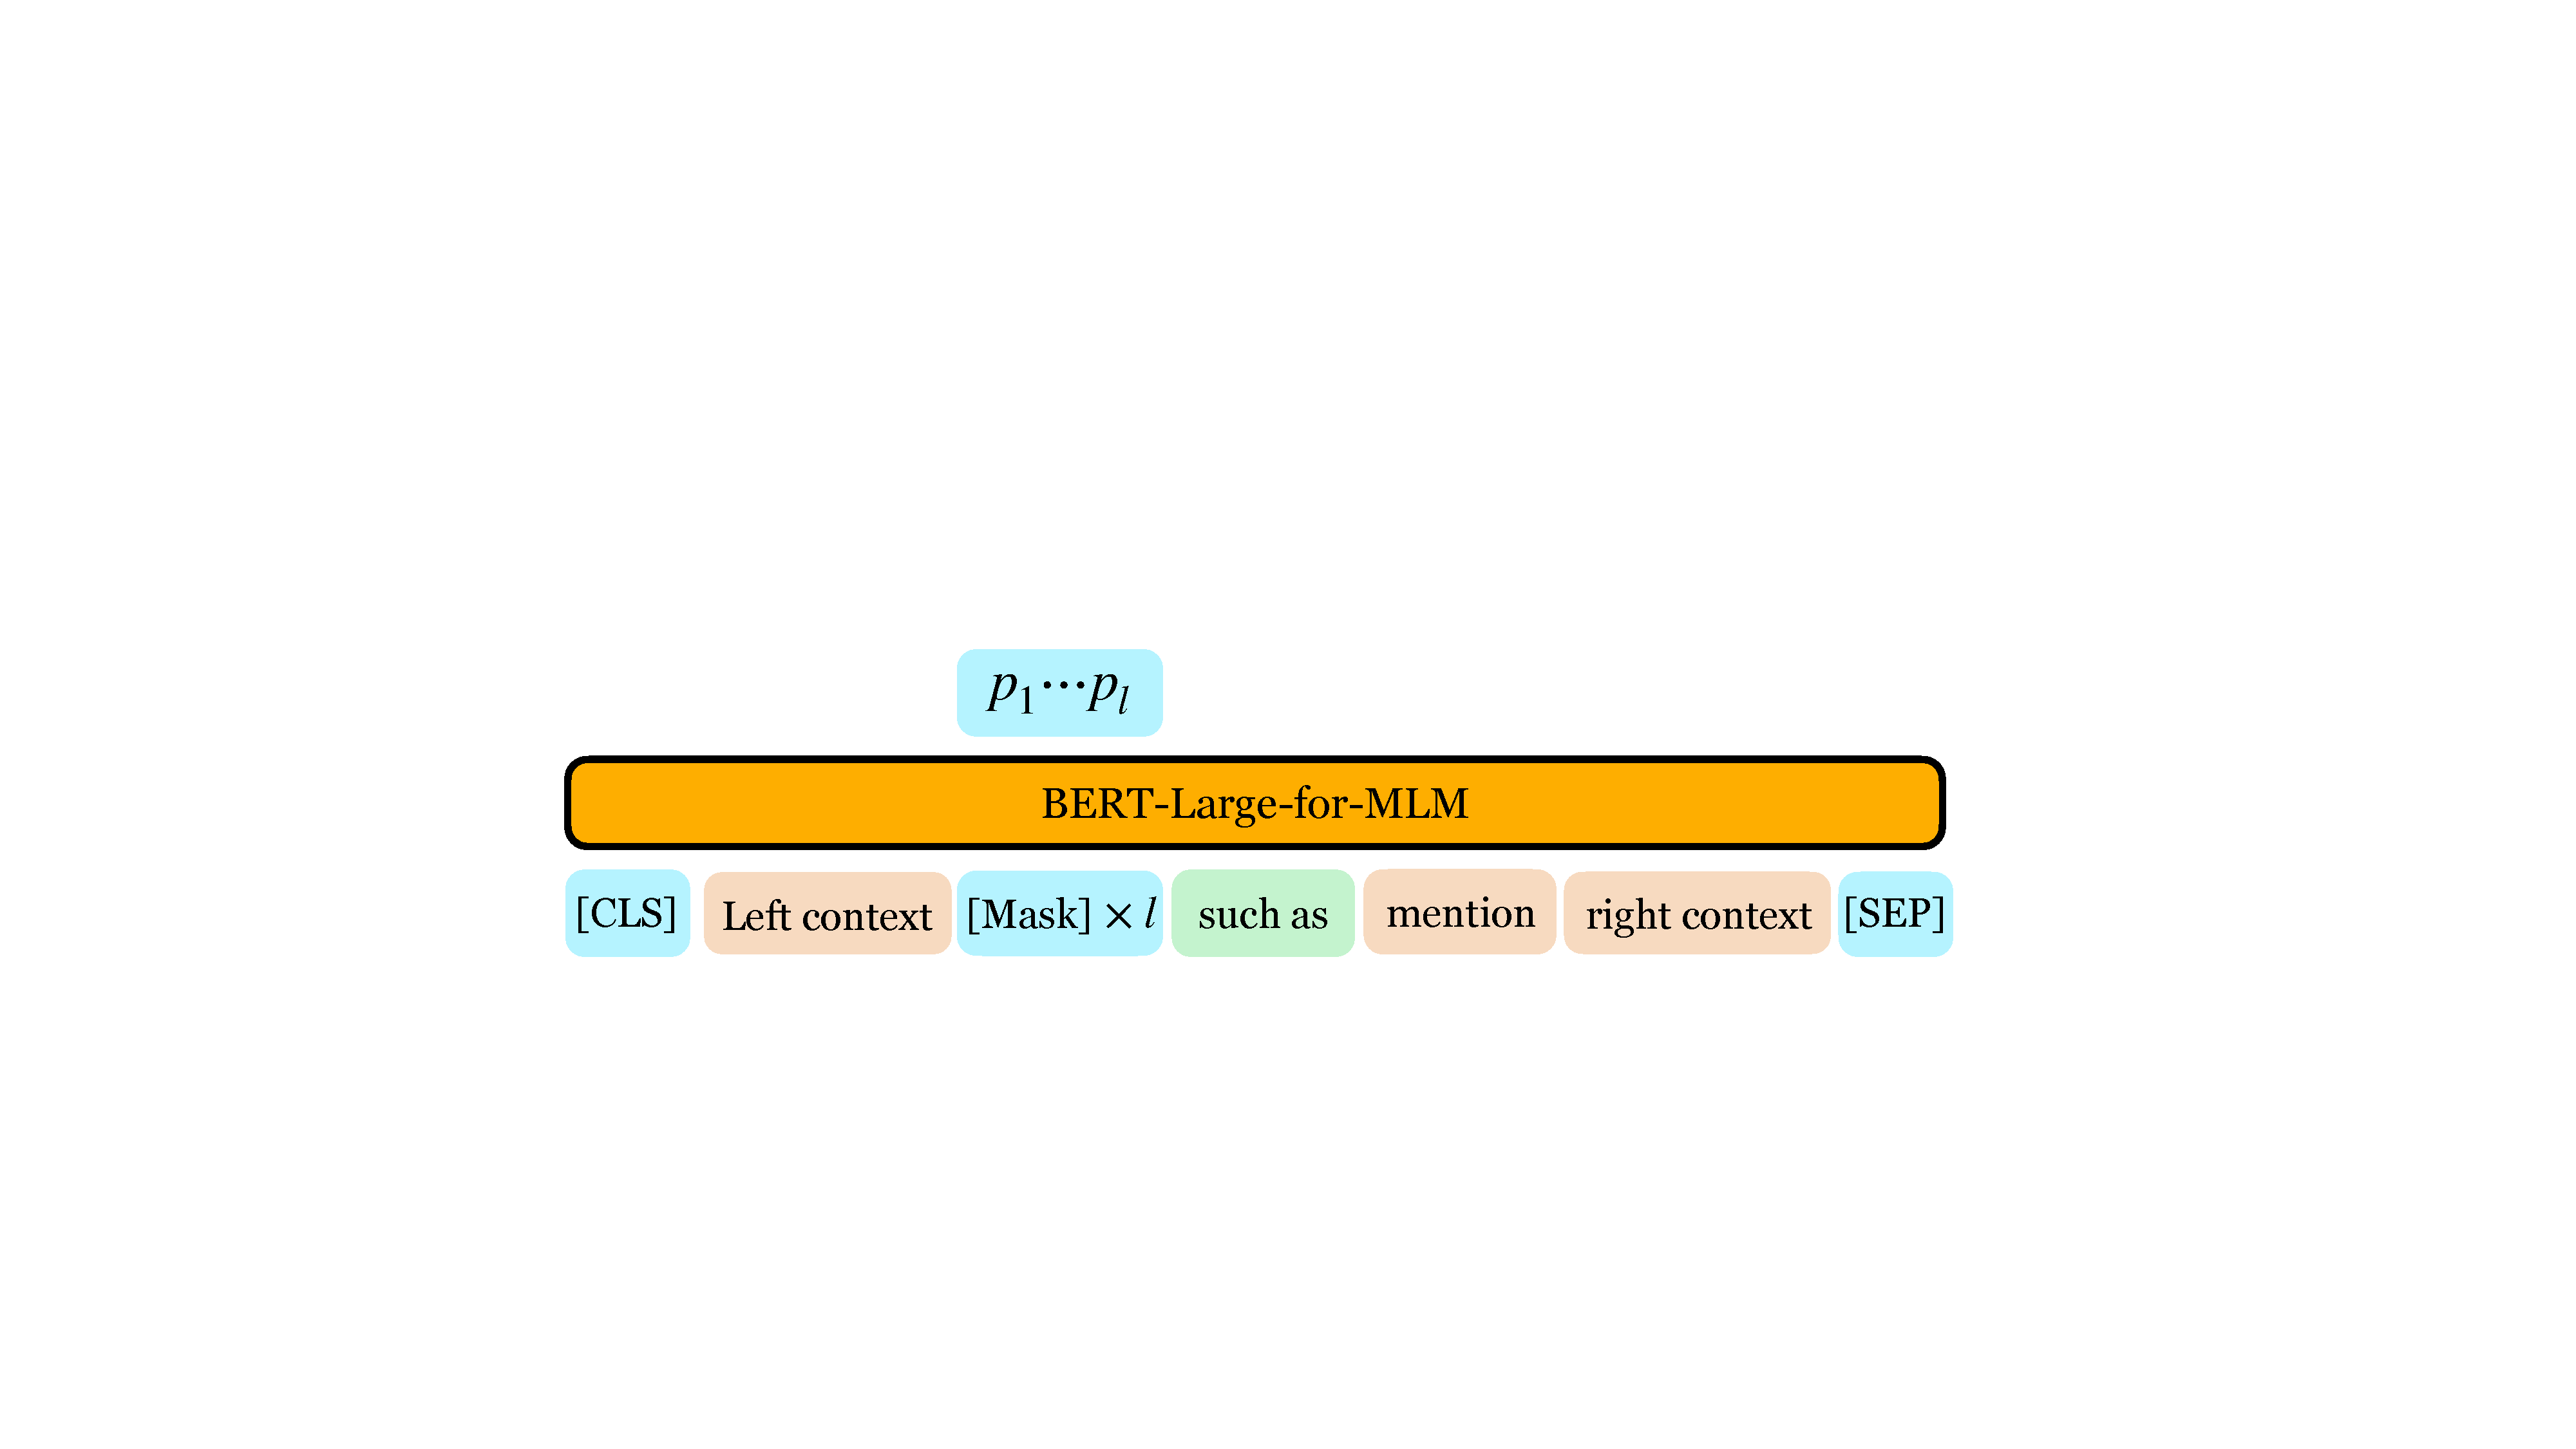
\includegraphics{src/img/prompt_recall.pdf}}
    \caption{Recall from MLM using prompts.}
    \label{fig:prompt_recall}
\end{figure}
where $c_i^l, c_i^r$ are left and right context of $m_i$, and \texttt{`such as'} is the template we use to induce types. The input is then fed into BERT-large-uncased\footnote{We use the PLM from \url{https://huggingface.co}} for masked language model to obtain the probabilities of subwords, the score of $y_j$ is calculated by $ s^{MLM}_{j} = (\sum_{n=1}^l \log p_n)/l$, where $p_l$ denotes the probability of subword $w_l$ predicted by the PLM. We rank all types by enumerating all possible $l$ and recall $K_2$ additional candidates that haven't been recalled by the recall stage and exact match. We found that the expand stage improves recalls and contributes to the performance in Sec. \ref{sec:exp_expand}.
\subsection{Filter Stage}
In the filter stage, we use the recall and expand method introduced above to efficiently generate type candidates $\mathcal{C}_i$ for data in the train, development, and test set. For training, $\mathcal{C}_i$ is used to produce positive and hard negative type candidates. For inference, $\mathcal{C}_i$ is the candidate pool for the trained filter models. Let $|\mathcal{C}_i|=K$ and $K$ is typically less than 256. 
\subsubsection{CE} A trivial idea is to train a CE model introduced in Sec. \ref{sec:vanilla_ce} to filter $\mathcal{C}_i$ instead of filtering the whole type set $\mathcal{Y}$. The positive type $y^{+}$ and negative $y^{\_}$ type are both sampled from $\mathcal{C}_{i}$ and are used for calculating marginal ranking loss. To infer types, we also recall and expand $K$ candidates and score these candidates by $K$ forward passes to predict types. As $K << |\mathcal{Y}|$, CE with our Recall-Expand-Filter paradigm is much faster than vanilla CE. However, it's still inefficient compared to MLC-like models that concurrently predict scores of all types in a single forward pass. For faster inference and training, we propose multi-candidate cross-encoders ({\bf \textsc{\name}}) and introduce them in the next section.

\section{Multi-Candidate Cross-Encoder (\name)}
\label{sec:ccf}
 In this section, we introduce {\bf \textsc{\name}} for filtering candidates in one forward pass and propose several variants. 
\subsection{Overall Introduction of \name}
As shown in Figure \ref{fig:ccf}, compared to CE that concatenates one candidate at a time, {\bf \textsc{\name}} models concatenate all candidates in $\mathcal{C}_i$ with the mention and context. The input is then fed into the PLM to obtain the hidden states of each candidate as their representation. Finally, we use an MLP to concurrently score all candidates.
\begin{equation}
\begin{aligned}
\bm{h}_{1:K}  &= \texttt{PLM}(\texttt{[CLS]} \ c_i \ \texttt{[SEP]}\  m_i \ \texttt{[SEP]} \ t_{1:K} \ )  \\
\bm{s}_{1:K}  &= \texttt{Linear}(\bm{h}_{1:K}) 
\end{aligned}
\end{equation}
where $t_{1:K}$ is the short for $t_1, \cdots, t_K$, and $t_j \in \mathcal{C}_i$. Similarly, $\bm{h}_{1:K}$ and $s_{1:K}$ are hidden representations and scores of corresponding candidates respectively. 

\paragraph{Training and Inference} For training, we found that all positive types are ranked very high in the training candidates, which is not the case for the development and test data. To prevent the filter model from overfitting the order of training candidates and only learning to predict the first several candidates, we keep permuting type candidates during training. Same as the MLC model mentioned in Sec. \ref{sec:mlc}, we use the Binary Cross-Entropy loss as the training objective and tune a threshold of probabilities on the development set for inference.

In the next subsection, we discuss different model configurations of {\bf \textsc{\name}} regarding the input formats of candidates and attention mechanisms.

\subsection{Different Input Formats of Candidates}
\paragraph{Average of type sub-tokens} We treat each type $t_j \in \mathcal{Y}$ as a new token $u_j$ and add it to the vocabulary of PLM. The static embedding (layer 0 embedding of PLM) of $u_j$ is properly initialized by the average static embedding of $t_j$'s sub-tokens. As type candidates are capsuled into single tokens, the candidate representation $t_j$ is simply the last hidden state of $u_j$. The reasons for representing each type as a single token is (1) The max sequence length allowed by most PLMs is limited to 512, compressing types into single tokens is position saving. (2) Types in {\bf \textsc{UFET}} are tokenized into $2.1$ sub-tokens in average (by RoBERTa's tokenizer). Compressing types will not lose too many type semantics.
\paragraph{Fixed-size sub-token block} To preserve more type semantics, we place each candidate into a fixed-sized block as shown in Figure \ref{fig:cand_block}. We found the fixed block size makes PLM easier to enable the parallel implementation of different attention mechanisms that we will introduce next. We use the first hidden state in the block as the candidate representation.
\begin{figure}[h]
    \centering
    \scalebox{0.3}{
    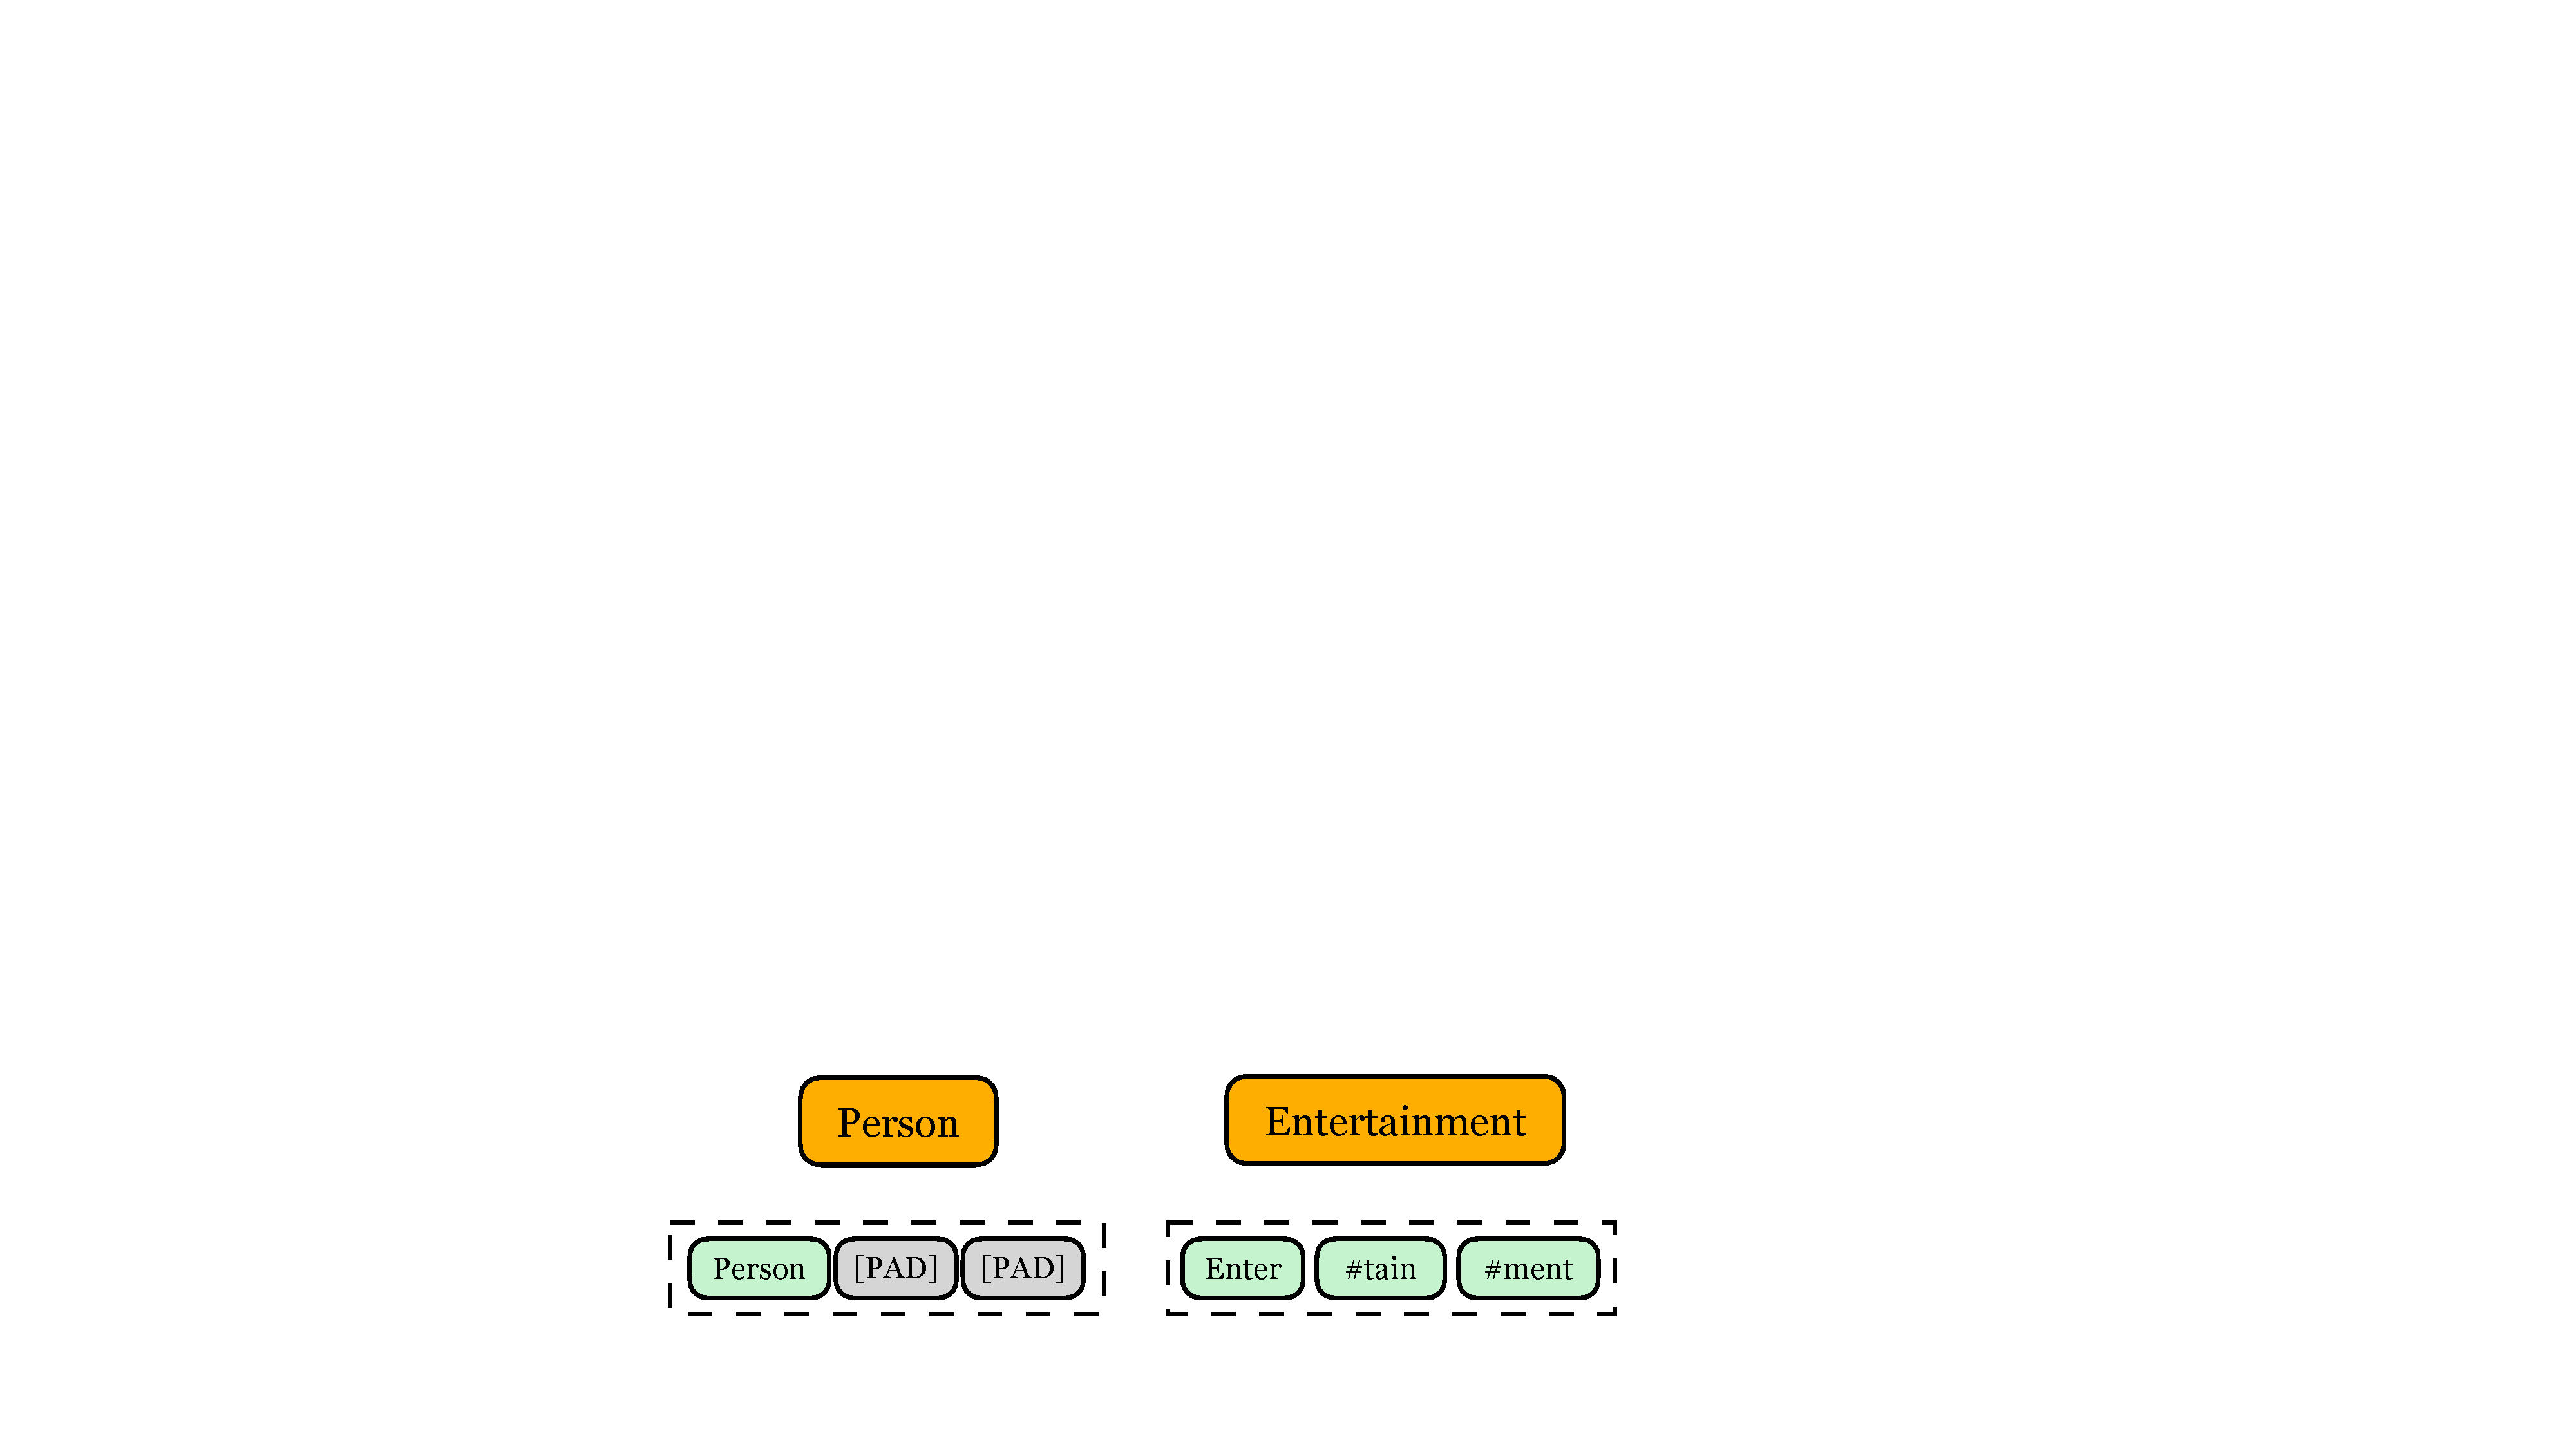
\includegraphics{src/img/cand_block.pdf}}
    \caption{Illustration of candidate block.}
    \label{fig:cand_block}
\end{figure}

\subsection{Attentions in \name}
\label{sec:attn}
There are four kinds of attention in {\bf \textsc{\name}} as shown in Figure \ref{fig:attn1}, sentence to sentence (S2S), sentence to candidates (S2C), candidate to sentence (C2S), and candidate to candidate (C2C). As we score candidates based on mention and its context, attention from candidates to the sentence (C2S) is necessary. However, the necessity of C2C, S2S, and S2C is questionable. As our analytical experiment in Sec. \ref{sec:analyze} shows, it is important for words in the sentence to attend to all candidates (S2C), and is useful to have self-attention in the sentence (S2S), but the attentions (C2C) between different candidates are unnecessary. Based on these findings, we propose a new variant of {\bf \textsc{\name}} that the C2C attention is discarded in computation as shown in the right part of Figure \ref{fig:attn1}. Let $L_S$ and $L_C$ be the number of sub-tokens used by the sentence and candidates respectively. We can formulate the attention query of the sentence as $\bm{Q}_S=[\bm{q}^s_{1};\cdots;\bm{q}^s_{L_S}] \in \mathbb{R}^{L_S \times D}$,  where $\bm{q}^s_i$ is the query vector of the $i$-th sub-token in the sentence, and $D$ is the embedding dimension. Similarly, the query of candidates is formulated as $\bm{Q}_C=[\bm{q}^c_{1};\cdots;\bm{q}^c_{L_C}] \in \mathbb{R}^{L_C \times D}$. When we treat candidates as average of sub-tokens, $\bm{q}^c_i$ is a $D$-dimensional vector, and when we use fixed-sized blocks to place candidates, $\bm{q}^c_i \in \mathbb{R}^{B \times D}$ is the concatenation of the query vectors in the $i$-th candidate block and $B$ is the number of sub-tokens in a block. The keys and values are defined similarly as $\bm{K}_C, \bm{V}_C, \bm{O}_C \in \mathbb{R}^{L_C \times D},  \bm{K}_S, \bm{V}_S, \bm{O}_S \in \mathbb{R}^{L_S \times D}$. The attention outputs are computed as:
\begin{align}
& \bm{O}_S  = \text{Softmax} \big( \frac{\bm{Q}_S [\bm{K}_S; \bm{K}_C]^T}{\sqrt{D}} \big) \cdot [\bm{V}_S; \bm{V}_C] \\
&[\bm{A}_{CS}; \bm{A}_{CC}]  = \text{Softmax} \big( \frac{[\bm{Q}_C \bm{K}_S^T; \bm{M}_C^T]}{\sqrt{D}} \big)  \\
&\bm{M}_C  =  [{\bm{q}_1^c}^T \bm{k}_1^c; \cdots; {\bm{q}_{L_C}^c}^T \bm{k}_{L_C}^c] \\
&\bm{A}_{CC} = [\bm{a}^c_{1}; \cdots; \bm{a}^c_{L_C}] \\
&\bm{O}_C = \bm{A}_{CS} \bm{V}_S + \sum_{j=1}^{L_C} \bm{a}_j \bm{v}^c_j
\end{align}
where $\bm{A}_{CC}$ is the intra-candidate or intra-block attention, and $\bm{a}_j^c$ is a scaler when we treat candidates as average of sub-tokens and is a $B \times B$ matrix when we represent candidates as blocks. The last step (Eq. 8) can be parallelly implemented by Einstein summation.
In most cases, candidate length $L_C$ is significantly larger than sentence length $L_S$. As a result, by ignoring the C2C attention, the inference speed is further improved because the time complexity of the attention is significantly reduced from $O(D(L_S+L_C)^2)$ to $O(D(L_S^2+2L_SL_C+B^2L_C))$. More importantly, the space complexity in attention also gets reduced from $O((L_S+L_C)^2)$ to $O(L_S^2+2L_SL_C))$, which allows us to filter more candidates concurrently. The improvement in space and time complexity by discarding C2C attention is more obvious when the number of candidates becomes larger.

\begin{figure}[h]
    \centering
    \scalebox{0.22}{
    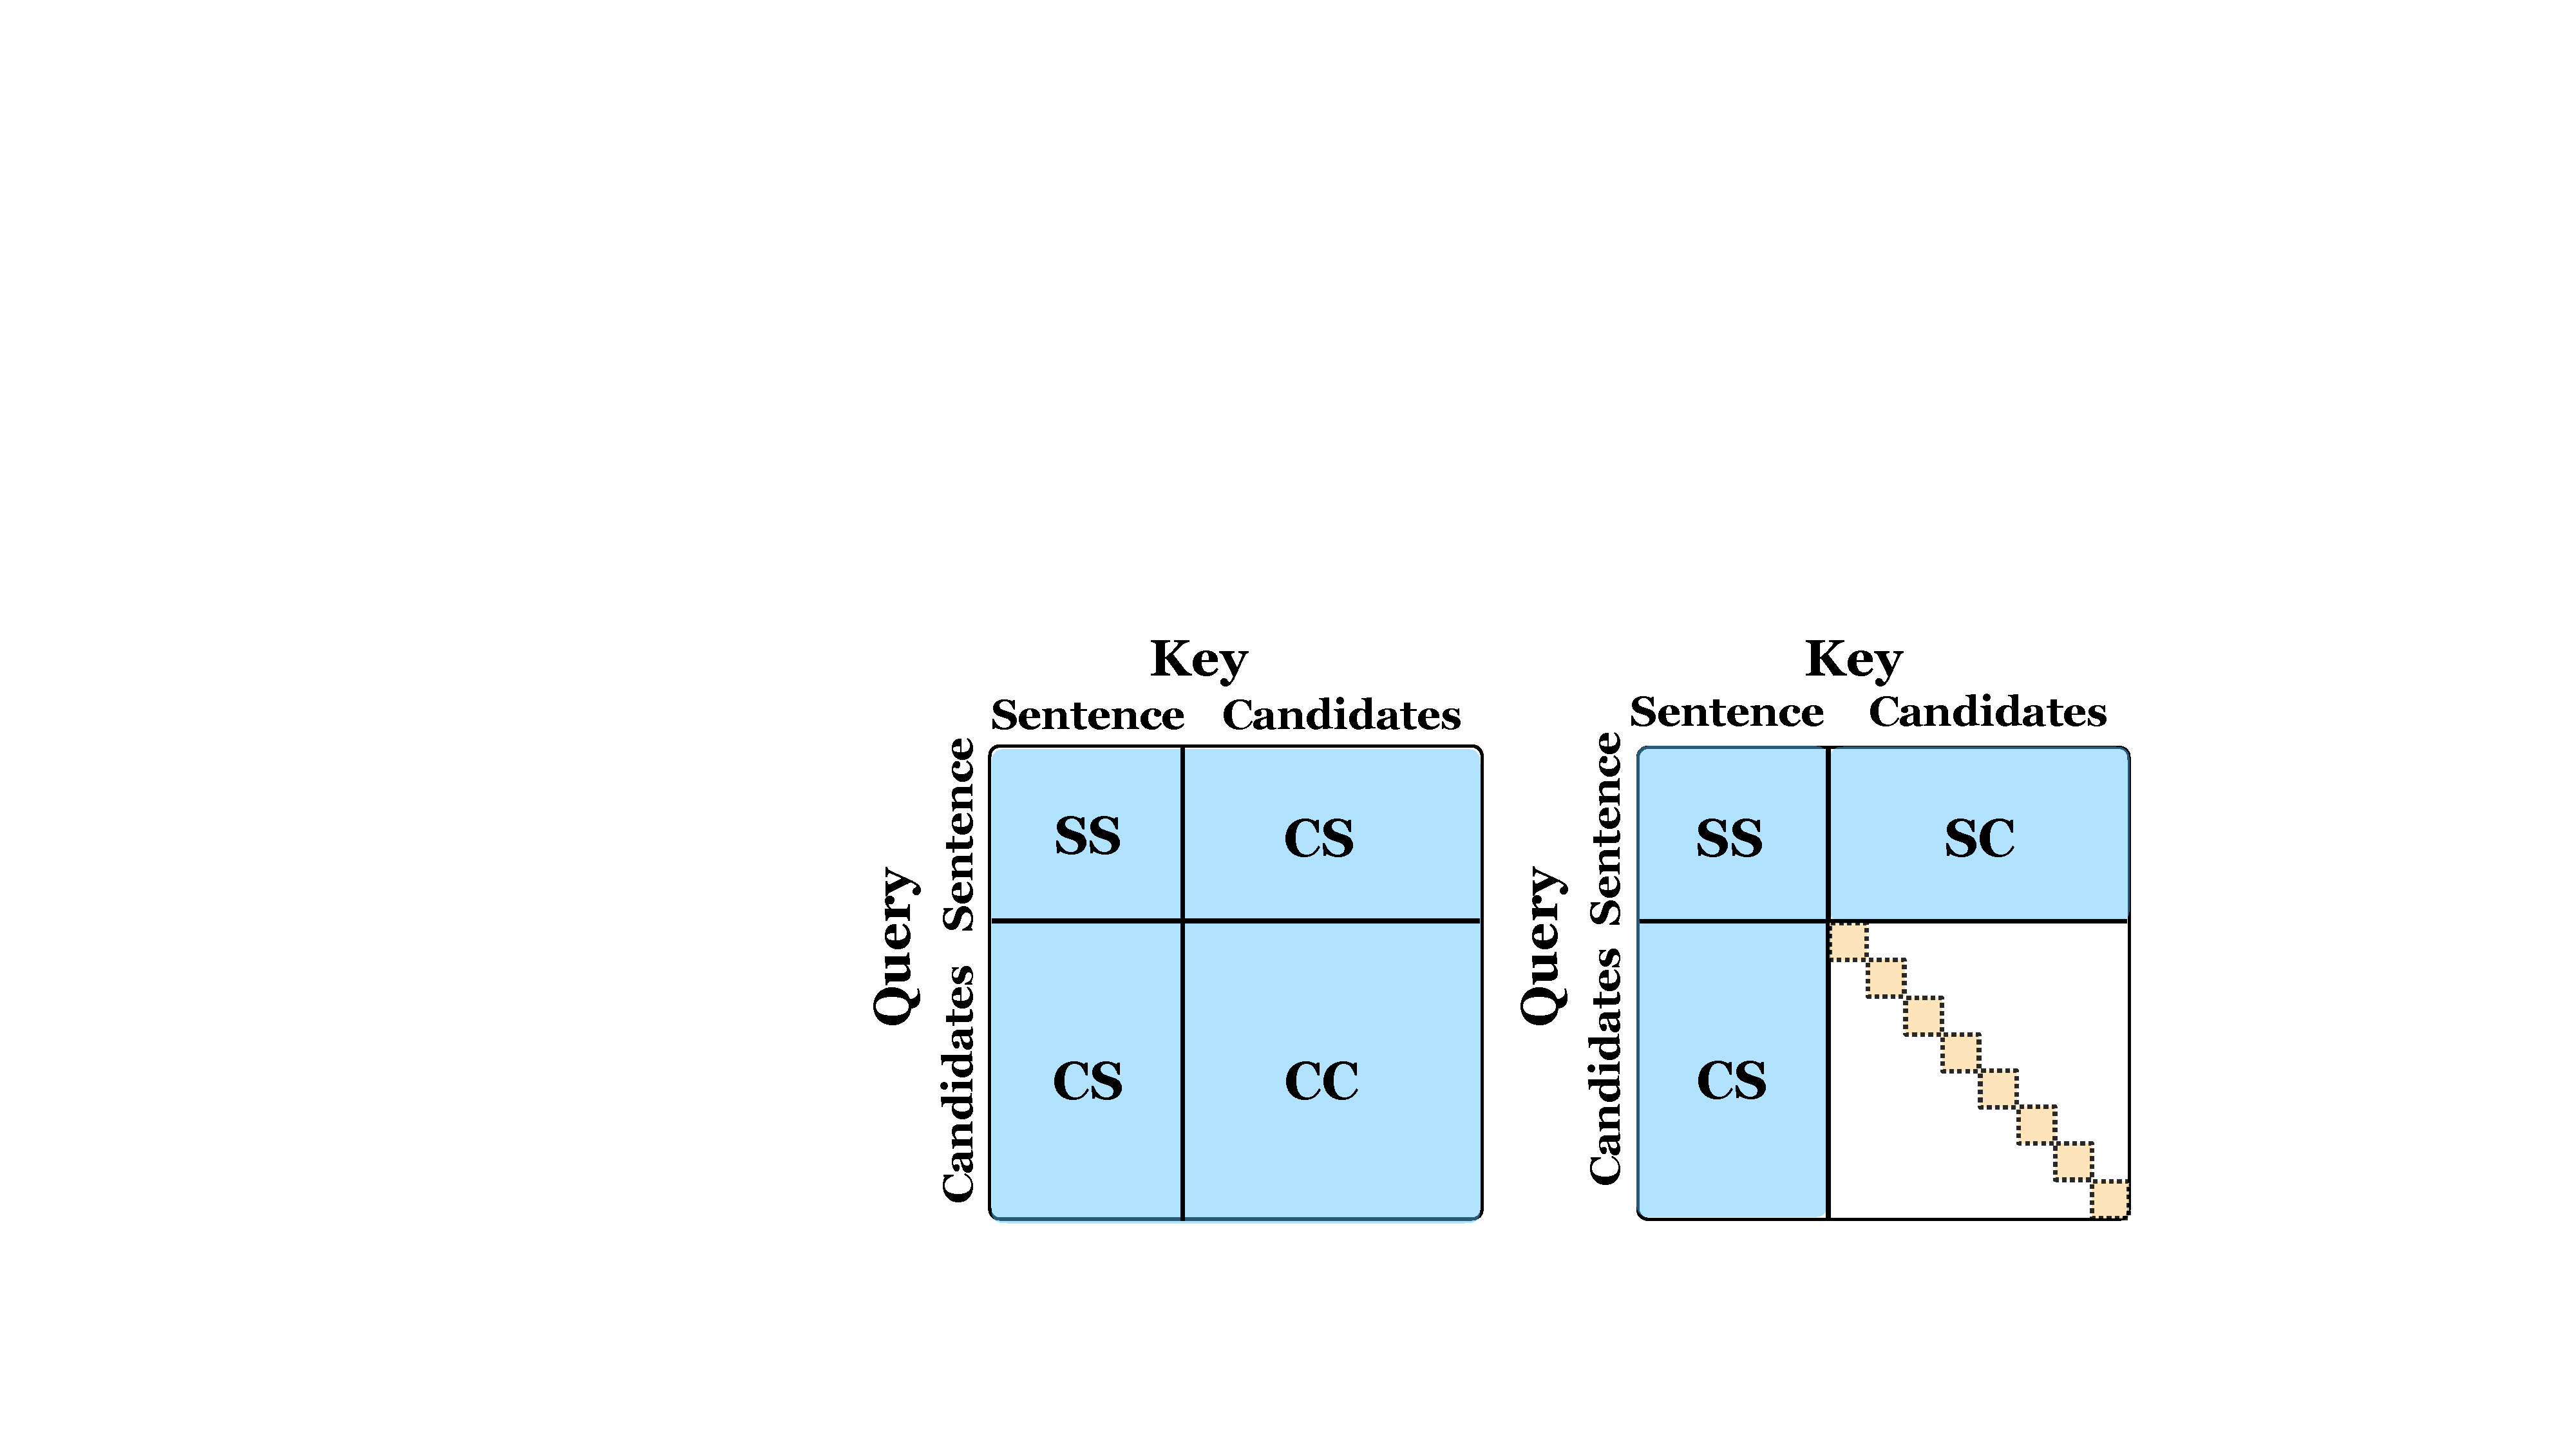
\includegraphics{src/img/attn_all.pdf}}
    \caption{Attentions in {\bf \textsc{\name}} (left), and {\bf \textsc{\name}}  without candidate-to-candidate (C2C) attention (right).}
    \label{fig:attn1}
\end{figure}